\section{Exercise: Estimating Speciation \& Extinction Rates}

\subsection{Introduction}

Models of speciation and extinction are fundamental to any phylogenetic analysis of macroevolutionary processes.
A prior describing the distribution of speciation events over time is critical to estimating phylogenies with branch lengths proportional to time.
Moreover, stochastic branching models allow for inference of speciation and extinction rates.
These inferences allow us to investigate key questions in evolutionary biology.

This tutorial describes how to specify simple branching-process models in \RevBayes;
two variants of the constant-rate birth-death process \citep{yule24,Kendall1948,thompson75,nee94,rannala96,yang97b}.
The probabilistic graphical model is given for each component of this exercise.
After each model is specified, you will estimate the marginal likelihood of the model and evaluate the relative support using Bayes factors.
Finally, you will estimate speciation and extinction rates using Markov chain Monte Carlo (MCMC) under the model supported by the data.


\subsection{The ``Observed'' Data}

\exs{Download data and \Rev~files from: 
\href{http://bit.ly/1tEDwTg}{http://bit.ly/1tEDwTg}}

The tree in this exercise contains a subset of the taxa resulting from the divergence-time analysis of 274 placental mammal species by \citet{dosReis2012}. 
The tree comprises all living bear species (8 taxa) plus two outgroups---the gray wolf and spotted seal.
Thus, the root of this tree represents the most-recent common ancestor of all living members of the suborder \href{http://en.wikipedia.org/wiki/Caniformia}{Caniformia} (Fig.~\ref{bearTree}). 
The phylogenetic relationships and speciation times are the median estimates reported by \citet{dosReis2012}. 
In this exercise, this time tree is treated as an ``observation'', and we are estimating parameters of the birth-death model without accounting for uncertainty in the time tree.

\exs{Open the tree \cl{data/bears\_dosReis.nex} in FigTree. }

\begin{figure}[h!]
\centering
\fbox{\includegraphics[width=3in]{\ResourcePath figures/bears_dosReis.eps}}
\caption{\small The relationships and median speciation times for bears and two outgroups estimated in the analysis by \citet{dosReis2012}.}
\label{bearTree}
\end{figure}

\bigskip
\section{Specifying Constant-Rate Birth-Death Models}\label{secModelSpec} 

Before evaluating the relative support for different models, we must first specify them in the \Rev~language.
In this section, we will walk through specifying three different variants of the birth-death process model and estimating the marginal likelihood under each one. 

\bigskip
\subsection{Pure-Birth Model}\label{yuleModSec}
%{\large \textcolor{mycol}{\textsc{Pure-Birth Model}}}

The simplest branching model is the \textit{pure-birth process} described by \citet{yule24}. 
Under this model, we assume at any instant in time, every lineage has the same speciation rate $\lambda$.
In its simplest form, the speciation rate remains constant over time. 
As a result, the waiting time between speciation events is exponential, where the rate of the exponential distribution is the product of the number of extant lineages ($n$) at that time and the speciation rate: $n\lambda$ \citep{yule24,aldous01,hartmann10}. 
The pure-birth branching model does not allow for lineage extinction (this is similar to population-level coalescent models). 
However, the model depends on a second parameter $\rho$ which is the probability of sampling a species in the present time as well as the time of the start of the process, whether that is the origin time or root age.
Therefore, the probabilistic graphical model of the pure-birth process is quite simple, where the observed time tree topology and node ages are conditional on the speciation rate, sampling probability, and root age (Fig.~\ref{yuleGMfig}).
\begin{figure}[h!]
\centering
\fbox{\includegraphics[width=3in]{\ResourcePath figures/yule_gm.eps}}
\caption{\small The graphical model representation of the pure-birth (Yule) process.}
\label{yuleGMfig}
\end{figure}

We can add hierarchical structure to this model and account for uncertainty in the value of the speciation rate by placing a hyperprior on $\lambda$ (Fig.~\ref{yuleGMfig2}). The graphical models in Figures \ref{yuleGMfig} and \ref{yuleGMfig2} demonstrate the simplicity of the Yule model. 
Ultimately, the pure birth model is just a special case of the birth-death process, where the extinction rate (typically denoted $\mu$) is a constant node with the value 0. 
\begin{figure}[h!]
\centering
\fbox{\includegraphics[width=4in]{\ResourcePath figures/yule_gm2.eps}}
\caption{\small The graphical model representation of the pure-birth (Yule) process, where the speciation rate is treated as a random variable drawn from an exponential distribution with rate parameter $\nu$.}
\label{yuleGMfig2}
\end{figure}

For this exercise, we will specify a Yule model, such that the speciation rate is a stochastic node, drawn from an exponential distribution as in Figure \ref{yuleGMfig2}.
In a Bayesian framework, we are interested in estimating the posterior probability of $\lambda$ given that we observe a time tree.
\begin{align}\label{bayesTher}
\mathbb{P}(\lambda \mid \Psi) &= \frac{\mathbb{P}(\Psi \mid \lambda)\mathbb{P}(\lambda \mid \nu)}{\mathbb{P}(\Psi)}
\end{align}
In this example, we have a phylogeny of all living bears plus two outgroup species, the gray wolf and spotted seal. 
We are treating the time tree $\Psi$ as an observation, thus clamping the model with an observed value.
The time tree we are conditioning the process on is taken from the analysis by \citet{dosReis2012} and shown in Figure \ref{bearTree}.
Furthermore, there are approximately 147 described caniform species, so we will fix the parameter $\rho$ to $10/147$.


\exs{The full Yule-model specification is in the file called \href{https://github.com/revbayes/revbayes/raw/development/tutorials/RB_TimeTree_Tutorials/RB_Diversification_Exercise/RB_diversification_files/RevBayes_scripts/m_Yule_bears.Rev}{\cl{m\_Yule\_bears.Rev}}.}

\subsubsection{Read the tree}

Begin by reading in the observed tree from Figure \ref{bearTree}. 

{\tt \begin{snugshade*}
\begin{lstlisting}
T <- readTrees("data/bears_dosReis.tre")[1]
\end{lstlisting}
\end{snugshade*}}

From this tree, we can get some helpful variables:
{\tt \begin{snugshade*}
\begin{lstlisting}
n_taxa <- T.ntips()
names <- T.names()
\end{lstlisting}
\end{snugshade*}}

Additionally, we can initialize an iterator variable for our vector of moves:
{\tt \begin{snugshade*}
\begin{lstlisting}
mi = 1 
\end{lstlisting}
\end{snugshade*}}

\subsubsection{Birth rate}

The model we are specifying only has three nodes (Fig.~\ref{yuleGMfig2}). 
We can specify the birth rate $\lambda$, the rate-parameter $\nu$ of the exponential hyperprior on $\lambda$, and the conditional dependency of the two parameters all in one line of \Rev~code.
{\tt \begin{snugshade*}
\begin{lstlisting}
birth_rate ~ dnExponential(0.1) 
\end{lstlisting}
\end{snugshade*}}
Here, the stochastic node called \cl{birth\_rate} represents $\lambda$ and the \cl{0.1} is the constant node $\nu$, given the value 0.1. 
Note that this value leads to an expected value for $\lambda$ of 10:
$$\mathbb{E}[\lambda]=\nu^{-1} = 10$$

To estimate the value of $\lambda$, we assign a proposal mechanism to operate on this node. 
In \RevBayes~these MCMC sampling algorithms are called \textit{moves}. 
We need to create a vector of moves and we can do this by using vector indexing and our pre-initialized iterator \cl{mi}.
We will use a scaling move on $\lambda$ called \cl{mvScale}.
{\tt \begin{snugshade*}
\begin{lstlisting}
moves[mi++] = mvScale(birth_rate,lambda=1,tune=true,weight=3)
\end{lstlisting}
\end{snugshade*}}

\subsubsection{Sampling probability}

Our prior belief is that we have sampled 10 out of 147 living caniform species. 
To account for this we can set the sampling parameter as a constant node with a value of 0.068
{\tt \begin{snugshade*}
\begin{lstlisting}
rho <- 0.068
\end{lstlisting}
\end{snugshade*}}


\subsubsection{Root age}

Any stochastic branching process must be conditioned on a time that represents the start of the process. 
Typically, this parameter is the \textit{origin time} and it is assumed that the process started with \textit{one} lineage. 
Thus, the origin of a birth-death process is the node that is \textit{ancestral} to the root node of the tree.
For macroevolutionary data, particularly without any sampled fossils, it is difficult to use the origin time.
To accommodate this, we can condition on the age of the root by assuming the process started with \textit{two} lineages that both originate at the time of the root.

We can get the value for the root from the \citet{dosReis2012} tree.

{\tt \begin{snugshade*}
\begin{lstlisting}
root_time <- treeHeight(T)
\end{lstlisting}
\end{snugshade*}}

\subsubsection{The time tree}

Now we have all of the parameters we need to specify the full pure-birth model. 
We can initialize the stochastic node representing the time tree.
Note that we set the \cl{mu} parameter to the constant value \cl{0.0}.
{\tt \begin{snugshade*}
\begin{lstlisting}
timetree ~ dnBDP(lambda=birth_rate, mu=0.0, rho=rho, rootAge=root_time, samplingStrategy="uniform", condition="nTaxa", nTaxa=n_taxa, names=names)\end{lstlisting}
\end{snugshade*}}

If you refer back to Equation \ref{bayesTher} and Figure \ref{yuleGMfig2}, the time tree $\Psi$ is the variable we observe, i.e., the data. 
We can set this in the \Rev~language by using the \cl{clamp()} function.
{\tt \begin{snugshade*}
\begin{lstlisting}
timetree.clamp(T)
\end{lstlisting}
\end{snugshade*}}
Here we are fixing the value of the time tree to our observed tree from \citet{dosReis2012}.
If we did not clamp this node, and ran MCMC, we would simply simulate time trees under the model.

Finally, we can create a workspace object of our whole model using the \cl{model()} function. 
Workspace objects are initialized using the \cl{=} operator. This distinguishes the objects used by the program
to run the MCMC analysis from the distinct nodes of our graphical model.
The model workspace objects makes it easy to work with the model in the \Rev~language and creates a wrapper around our model DAG. 
Because our model is a directed, acyclic graph (DAG), we only need to give the model wrapper function a single node and it does the work to find all the other nodes through their connections.
{\tt \begin{snugshade*}
\begin{lstlisting}
mymodel = model(birth_rate)
\end{lstlisting}
\end{snugshade*}}

The \cl{model()} function traversed all of the connections and found all of the nodes we specified. 
We can now visualize our graphical model using the \cl{.graph()} member method of the model object. 
This function writes a file in the \href{http://en.wikipedia.org/wiki/DOT_(graph_description_language)}{DOT graph-description language}.
The contents of this file describes the nodes and edges of the model DAG and can be read by an interpreter program called \href{http://www.graphviz.org/}{Graphviz}.
First create the model graph file using the \cl{.graph()} method. Set the flag for extra output (good for development debugging) to false: \cl{verbose=false}.
And specify a \href{http://web.njit.edu/~kevin/rgb.txt.html}{named RBG color} for the background (for this graph, we like \cl{"honeydew2"}). 
{\tt \begin{snugshade*}
\begin{lstlisting}
mymodel.graph("output/m_Yule_bears_GM.dot", verbose=false, bg="honeydew2")
\end{lstlisting}
\end{snugshade*}}

Open the \cl{output/m\_Yule\_bears\_GM.dot} file in the \href{http://www.graphviz.org/}{Graphviz} program or paste the contents in an online viewer:
\begin{itemize}[noitemsep,nolistsep]
  \item \href{http://graphviz-dev.appspot.com/}{http://graphviz-dev.appspot.com/}
  \item \href{http://stamm-wilbrandt.de/GraphvizFiddle/}{http://stamm-wilbrandt.de/GraphvizFiddle/}
\end{itemize}

Your graph should look like the one depicted in Figure \ref{yuleGMGVfig}.
Compare this figure to the model in Figure \ref{yuleGMfig2}.
You should notice that there are two extra nodes in the Figure \ref{yuleGMGVfig}. 
The constant node with the value \cl{0} connected to the \cl{birth\_rate} stochastic node represents the \cl{offset} variable of the exponential distribution which is given the default value of 0 when no offset is provided. 
Additionally, there is a nameless constant node with the value of \cl{0} pointing into the clamped \cl{timetree} stochastic node. 
This constant node represents the death rate, \cl{mu}, which we set to \cl{0} when we initialized \cl{timetree} using the \cl{dnBDP()} constructor function.
Viewing the model graph is helpful for identifying any problems prior to running MCMC. 
\begin{figure}[h!]
\centering
\fbox{\includegraphics[width=3in]{\ResourcePath figures/m_Yule_bears_GM.eps}}
\caption{\small The graphical model representation of the pure-birth (Yule) process generated using the DOT language and the \href{http://www.graphviz.org/}{Graphviz} program.}
\label{yuleGMGVfig}
\end{figure}


\subsubsection{Estimating the marginal likelihood of the model}

With a fully specified model, we can set up the \cl{powerPosterior()} analysis to create a file of `powers' and likelihoods from which we can estimate the marginal likelihood using stepping-stone or path sampling. 
This method computes a vector of powers from a beta distribution, then executes an MCMC run for each power step while raising the likelihood to that power. In this implementation, the vector of powers starts with 1, sampling the likelihood close to the posterior and incrementally sampling closer and closer to the prior as the power decreases. 

\exs{The \Rev~file for performing this analysis: \href{https://github.com/revbayes/revbayes/raw/development/tutorials/RB_TimeTree_Tutorials/RB_Diversification_Exercise/RB_diversification_files/RevBayes_scripts/mlnl_Yule_bears.Rev}{\cl{mlnl\_Yule\_bears.Rev}}.}

First, we create the variable containing the power posterior. This requires us to provide a model and vector of moves, as well as an output file name. The \cl{cats} argument sets the number of power steps.
{\tt \begin{snugshade*}
\begin{lstlisting}
pow_p = powerPosterior(mymodel, moves, "output/Yule_bears_powp.out", cats=50) 
\end{lstlisting}
\end{snugshade*}}

We can start the power posterior by first burning in the chain and and discarding the first 10000 states.  
{\tt \begin{snugshade*}
\begin{lstlisting}
pow_p.burnin(generations=10000,tuningInterval=1000)
\end{lstlisting}
\end{snugshade*}}

Now execute the run with the \cl{.run()} function:
{\tt \begin{snugshade*}
\begin{lstlisting}
pow_p.run(generations=1000)  
\end{lstlisting}
\end{snugshade*}}

Once the power posteriors have been saved to file, create a stepping stone sampler. This function can read any file of power posteriors and compute the marginal likelihood using stepping-stone sampling. 
{\tt \small \begin{snugshade*}
\begin{lstlisting}
ss = steppingStoneSampler(file="output/Yule_bears_powp.out", powerColumnName="power", likelihoodColumnName="likelihood")
\end{lstlisting}
\end{snugshade*}}

Compute the marginal likelihood under stepping-stone sampling using the member function \cl{marginal()} of the \cl{ss} variable and record the value in Table \ref{ssTable}.
{\tt \begin{snugshade*}
\begin{lstlisting}
ss.marginal() 
\end{lstlisting}
\end{snugshade*}}

Path sampling is an alternative to stepping-stone sampling and also takes the same power posteriors as input. 
{\tt \small \begin{snugshade*}
\begin{lstlisting}
ps = pathSampler(file="output/Yule_bears_powp.out", powerColumnName="power", likelihoodColumnName="likelihood")
\end{lstlisting}
\end{snugshade*}}

Compute the marginal likelihood under stepping-stone sampling using the member function \cl{marginal()} of the \cl{ps} variable and record the value in Table \ref{ssTable}.
{\tt \begin{snugshade*}
\begin{lstlisting}
ps.marginal() 
\end{lstlisting}
\end{snugshade*}}

\bigskip
\section{Birth-Death Process}\label{birthDeathSec}

The pure-birth model does not account for  extinction, thus it assumes that every lineage at the start of the process will have sampled descendants at time 0.
This assumption is fairly unrealistic for most phylogenetic datasets on a macroevolutionary time scale since the fossil record provides evidence of extinct lineages.
\citet{kendall48} described a more general branching process model to account for lineage extinction called the \textit{birth-death process}.
Under this model, at any instant in time, every lineage has the same rate of speciation $\lambda$ and the same rate of extinction $\mu$.
This is the \textit{constant-rate} birth-death process, which considers the rates constant over time and over the tree \citep{nee94}.
Importantly, this model assumes that all of the extant descendants of the process have been sampled at time 0.

\citet{yang97b} derived the probability of time trees under an extension of the birth-death model that accounts for incomplete sampling of the tips (Fig.~\ref{bdrGMFig1}). 
Under this model, the parameter $\rho$ accounts for the probability of sampling in the present time, and because it is a probability, this parameter can only take values between 0 and 1. 
\begin{figure}[h!]
\centering
\fbox{\includegraphics[width=3in]{\ResourcePath figures/simple_BD_gm_root.eps}}
\caption{\small The graphical model representation of the birth-death process with uniform sampling and conditioned on the root age.}
\label{bdrGMFig1}
\end{figure}

Ultimately, it is difficult to formulate prior densities on rate parameters, particularly when our uncertainty in the values of the speciation and extinction rates is quite large. 
Furthermore, without sampling the process back in time, it is difficult to estimate extinction. 
Thus, we can re-parameterize the birth-death process to account for these issues.
In this parameterization, we use the net diversification rate $d$ and the turnover rate $r$ (also called relative extinction rate) instead of the $\lambda$, $\mu$ parameters.
\begin{center}
\begin{tabular}{rcl}
$d=\lambda-\mu$ & \hspace{6mm} & Net diversification rate\\
$r=\mu / \lambda$ & & Turnover\\
\end{tabular} 
\end{center}
Importantly, we can recover $\lambda$ and $\mu$ via: 
\begin{equation}\label{lambdamufxns}
\lambda=\frac{d}{1-r}, \quad \mu=\frac{rd}{1-r}.
\end{equation}
Thus, $\lambda$ and $\mu$ are deterministic nodes, transformed from $d$ and $r$. 
By using the diversification and turnover parameters, we now have another variable, $r$ that can only take values between 0 and 1.
This is because, under the constant-rate birth-death process, $\mu$ can never be greater than $\lambda$ (Fig.~\ref{bdrGMFig2}). 
Note that if $\mu=0$, then $d = \lambda$ in this parameterization.


\begin{figure}[h!]
\centering
\fbox{\includegraphics[width=3in]{\ResourcePath figures/cBDR_gm.eps}}
\caption{\small The graphical model representation of the birth-death process with uniform sampling parameterized using the diversification and turnover.}
\label{bdrGMFig2}
\end{figure}

In this model, we will specify an exponential prior density on $d$ and a beta prior on $r$.
There are approximately 147 described caniform species, so we will fix the parameter $\rho$ to $10/147$.

\exs{The full birth-death, fixed sampling model specification is in the file called \href{https://github.com/revbayes/revbayes/raw/development/tutorials/RB_TimeTree_Tutorials/RB_Diversification_Exercise/RB_diversification_files/RevBayes_scripts/m_BD_bears.Rev}{\cl{m\_BD\_bears.Rev}}.}


\subsection{Clear the workspace and read the tree}

It is best to remove all of the previous model variables created in the previous section.
{\tt \begin{snugshade*}
\begin{lstlisting}
clear()
\end{lstlisting}
\end{snugshade*}}

Now read in the observed tree from Figure \ref{bearTree}. 
{\tt \begin{snugshade*}
\begin{lstlisting}
T <- readTrees("data/bears_dosReis.tre")[1]
\end{lstlisting}
\end{snugshade*}}

Initialize the useful variables:
{\tt \begin{snugshade*}
\begin{lstlisting}
n_taxa <- T.ntips()
names <- T.names()
mi = 1 
\end{lstlisting}
\end{snugshade*}}

\subsection{Diversification and turnover}

The diversification and turnover are the parameters which we will treat as stochastic nodes in our model. 
We will assume an exponential prior on \cl{diversification} and assign it a scale move.
{\tt \begin{snugshade*}
\begin{lstlisting}
diversification ~ dnExponential(10.0) 
moves[mi++] = mvScale(diversification,lambda=1.0,tune=true,weight=3.0) 
\end{lstlisting}
\end{snugshade*}}

The \cl{turnover} parameter can only take values between 0 and 1, thus we will assume a beta prior on this parameter and sample from the posterior distribution using a scale move.
{\tt \begin{snugshade*}
\begin{lstlisting}
turnover ~ dnBeta(2.0, 2.0) 
moves[mi++] = mvSlide(turnover,delta=1.0,tune=true,weight=3.0)
\end{lstlisting}
\end{snugshade*}}

\subsection{Birth rate and death rate}

The birth and death rates are both deterministic nodes. 
Refer to Equation \ref{lambdamufxns}. Note that both the birth rate and death rate are functions of $d$ and $r$.

Because our variable transformations use the \cl{-} operator, we must additionally use the \cl{abs()} function to ensure that the rates are of type \cl{RealPos}, which is required by the birth-death process model.
{\tt \begin{snugshade*}
\begin{lstlisting}
birth_rate := abs(diversification / (1.0 - turnover))
\end{lstlisting}
\end{snugshade*}}

{\tt \begin{snugshade*}
\begin{lstlisting}
death_rate := abs(turnover * diversification / (1.0 - turnover))
\end{lstlisting}
\end{snugshade*}}

\subsection{The sampling probability}

If we assume that the 147 described caniform species represent all of the living caniforms on Earth, then it is quite reasonable to fix the parameter $\rho$ to a known value.
{\tt \begin{snugshade*}
\begin{lstlisting}
rho <- 0.068
\end{lstlisting}
\end{snugshade*}}

\subsection{Root age}

Get the value for the root from the \citet{dosReis2012} tree.

{\tt \begin{snugshade*}
\begin{lstlisting}
root_time <- treeHeight(T)
\end{lstlisting}
\end{snugshade*}}

\subsection{The time tree}

Initialize the stochastic node representing the time tree.
{\tt \begin{snugshade*}
\begin{lstlisting}
timetree ~ dnBDP(lambda=birth_rate, mu=death_rate, rootAge=root_time, rho=rho, samplingStrategy="uniform", condition="nTaxa", nTaxa=n_taxa, names=names)
\end{lstlisting}
\end{snugshade*}}

Since we are computing the likelihood on the \citet{dosReis2012} tree, we can consider this time tree as an observation and clamp the stochastic node.
{\tt \begin{snugshade*}
\begin{lstlisting}
timetree.clamp(T)
\end{lstlisting}
\end{snugshade*}}

Now set the workspace model variable.
{\tt \begin{snugshade*}
\begin{lstlisting}
mymodel = model(diversification)
\end{lstlisting}
\end{snugshade*}}

{\tt \begin{snugshade*}
\begin{lstlisting}
mymodel.graph("output/m_BD_bears_GM.dot", bg="LightSteelBlue2")
\end{lstlisting}
\end{snugshade*}}

\begin{figure}[h!]
\centering
\fbox{\includegraphics[width=3in]{\ResourcePath figures/m_BD_bears_GM.eps}}
\caption{\small The graphical model representation of the birth-death process.}
\label{BDGMGVfig}
\end{figure}



\subsection{Estimating the marginal likelihood of the model}

\exs{The \Rev~file for performing this analysis: \href{https://github.com/revbayes/revbayes/raw/development/tutorials/RB_TimeTree_Tutorials/RB_Diversification_Exercise/RB_diversification_files/RevBayes_scripts/mlnl_BD_bears.Rev}{\cl{mlnl\_BD\_bears.Rev}}.}

{\tt \begin{snugshade*}
\begin{lstlisting}
pow_p = powerPosterior(mymodel, moves, "output/BD_bears_powp.out", cats=50) 
pow_p.burnin(generations=10000,tuningInterval=1000)
pow_p.run(generations=1000)  
\end{lstlisting}
\end{snugshade*}}

Compute the marginal likelihood under stepping-stone sampling using the member function \cl{marginal()} of the \cl{ss} variable and record the value in Table \ref{ssTable}.
{\tt \small \begin{snugshade*}
\begin{lstlisting}
ss = steppingStoneSampler(file="output/BD_bears_powp.out", powerColumnName="power", likelihoodColumnName="likelihood")
ss.marginal() 
\end{lstlisting}
\end{snugshade*}}

Compute the marginal likelihood under stepping-stone sampling using the member function \cl{marginal()} of the \cl{ps} variable and record the value in Table \ref{ssTable}.
{\tt \small \begin{snugshade*}
\begin{lstlisting}
ps = pathSampler(file="output/BD_bears_powp.out", powerColumnName="power", likelihoodColumnName="likelihood")
ps.marginal() 
\end{lstlisting}
\end{snugshade*}}



\bigskip
\section{Compute Bayes Factors and Select Model}


Now that we have estimates of the marginal likelihood under each of our different models, we can evaluate their relative plausibility using Bayes factors.
Use Table \ref{ssTable} to summarize the marginal log-likelihoods estimated using the stepping-stone and path-sampling methods.

Phylogenetics software programs log-transform the likelihood to avoid \href{http://en.wikipedia.org/wiki/Arithmetic_underflow}{underflow}, because multiplying likelihoods results in numbers that are too small to be held in computer memory.
Thus, we must calculate the ln-Bayes factor (we will denote this value $\mathcal{K}$):
\begin{align}\label{LNbfFormula}
\mathcal{K}=\ln[BF(M_0,M_1)] = \ln[\mathbb{P}(\mathbf X \mid M_0)]-\ln[\mathbb{P}(\mathbf X \mid M_1)],
\end{align}
where $\ln[\mathbb{P}(\mathbf X \mid M_0)]$ is the \textit{marginal lnL} estimate for model $M_0$. 
The value resulting from equation \ref{LNbfFormula} can be converted to a raw Bayes factor by simply taking the exponent of $\cal{K}$
\begin{align}\label{LNbfFormula2}
BF(M_0,M_1) = e^{\cal{K}}.
\end{align}
Alternatively, you can interpret the strength of evidence in favor of $M_0$ using the $\cal{K}$ and skip equation \ref{LNbfFormula2}. 
In this case, we evaluate the $\cal{K}$ in favor of model $M_0$ against model $M_1$ so that:
\begin{center}
\begin{tabular}{l}
if $\mathcal{K} > 1$, then model $M_0$ wins\\
if $\mathcal{K} < -1$, then model $M_1$ wins.
\end{tabular}
\end{center}
Thus, values of $\mathcal{K}$ around 0 indicate ambiguous support. 


Using the values you entered in Table \ref{ssTable} and equation \ref{LNbfFormula},  calculate the ln-Bayes factors (using $\mathcal{K}$) for the different model comparisons. 
Enter your answers in Table \ref{ssTable} using the stepping-stone and the path-sampling estimates of the marginal log likelihoods. 

\begin{Form}
\begin{table}[h!]
\centering
\caption{\small Marginal likelihoods and Bayes factors$^*$.}
\begin{tabular}{l c c c c}
\hline
\multicolumn{1}{l}{\textbf{Estimate}} & \multicolumn{1}{r}{\hspace{3mm}} & \multicolumn{1}{c}{\textit{Stepping-stone}} & \multicolumn{1}{r}{\hspace{3mm}} & \multicolumn{1}{c}{\textit{Path sampling}} \\ 
\hline
\ref{yuleModSec} Marginal likelihood Yule ($M_0$) & \hspace{15mm} & \TextField[name=ml7,backgroundcolor={.85 .85 .85},color={1 0 0},height=4ex]{}  & \hspace{15mm} & \TextField[name=ml8,backgroundcolor={.85 .85 .85},color={0 0 1},height=4ex]{} \\
\hline
\ref{birthDeathSec} Marginal likelihood birth-death ($M_1$) & \hspace{3mm} & \TextField[name=ml9,backgroundcolor={.85 .85 .85},color={1 0 0},height=4ex]{} & \hspace{3mm} & \TextField[name=ml10,backgroundcolor={.85 .85 .85},color={0 0 1},height=4ex]{} \\
\hline
Eq.~\ref{LNbfFormula}: $BF(M_0,M_1)$ & \hspace{3mm} &  \TextField[name=ml11,backgroundcolor={.85 .85 .85},color={1 0 0},height=4ex]{} & \hspace{3mm} & \TextField[name=ml12,backgroundcolor={.85 .85 .85},color={0 0 1},height=4ex]{} \\
\hline
Supported model? & \hspace{3mm} &  \TextField[name=ml13,backgroundcolor={1 .85 .85},color={1 0 0},height=4ex]{} & \hspace{3mm} & \TextField[name=ml14,backgroundcolor={.85 .85 1},color={0 0 1},height=4ex]{} \\
\hline
{\footnotesize{$^*$you can edit this table}}\\
\end{tabular}
\label{ssTable}
\end{table}
\end{Form}

Do these data support a model without extinction ($\mu=0$)? %\TextField[name=ml13,backgroundcolor={1 .85 .85},color={1 0 0},height=4ex]{}

\bigskip
\section{Estimate Speciation and Extinction Rates}

After comparing the marginal likelihoods using Bayes factors, you will discover which model is best supported by the data. 
With this model, we can now estimate posterior probability of the the global rate of speciation (and extinction if the birth-death model is used) given our observed tree.
\begin{align}\label{bayesTher2}
\mathbb{P}(\lambda, \mu \mid \Psi) &= \frac{\mathbb{P}(\Psi \mid \lambda, \mu)\mathbb{P}(d \mid \nu)\mathbb{P}(r \mid \alpha, \beta)}{\mathbb{P}(\Psi)}
\end{align}


\exs{The \Rev~file for performing this analysis: \href{https://github.com/revbayes/revbayes/raw/development/tutorials/RB_TimeTree_Tutorials/RB_Diversification_Exercise/RB_diversification_files/RevBayes_scripts/mcmc_BD_bears.Rev}{\cl{mcmc\_BD\_bears.Rev}} or  \href{https://github.com/revbayes/revbayes/raw/development/tutorials/RB_TimeTree_Tutorials/RB_Diversification_Exercise/RB_diversification_files/RevBayes_scripts/mcmc_Yule_bears.Rev}{\cl{mcmc\_Yule\_bears.Rev}}.}


\subsection{Clear the workspace and load the preferred model}

It is best to remove all of the previous model variables created in the previous section.
{\tt \begin{snugshade*}
\begin{lstlisting}
clear()
\end{lstlisting}
\end{snugshade*}}


Now read in the observed tree from Figure \ref{bearTree}. 
{\tt \begin{snugshade*}
\begin{lstlisting}
T <- readTrees("data/bears_dosReis.tre")[1]
\end{lstlisting}
\end{snugshade*}}

Initialize the useful variables:
{\tt \begin{snugshade*}
\begin{lstlisting}
n_taxa <- T.ntips()
names <- T.names()
mi = 1 
\end{lstlisting}
\end{snugshade*}}



Source the model file of your favorite model ($* = $ \cl{Yule} or \cl{BD}).
{\tt \begin{snugshade*}
\begin{lstlisting}
source("RevBayes_scripts/m_*_bears.Rev")
\end{lstlisting}
\end{snugshade*}}

{\tt \begin{snugshade*}
\begin{lstlisting}
mymodel = model(birth_rate)
\end{lstlisting}
\end{snugshade*}}


\subsection{Set up parameter monitors}


{\tt \begin{snugshade*}
\begin{lstlisting}
monitors[1] = mnFile(filename="output/BDR_mcmc_bears.log",printgen=10, diversification, birth_rate, turnover, death_rate)
monitors[2] = mnScreen(printgen=1000, birth_rate)
\end{lstlisting}
\end{snugshade*}}

Note that if your preferred model was the Yule process, then you would only have the \cl{birth\_rate} parameter listed in the \cl{mnFile} monitor.

\subsection{Run MCMC}

{\tt \begin{snugshade*}
\begin{lstlisting}
mymcmc = mcmc(mymodel, monitors, moves)
\end{lstlisting}
\end{snugshade*}}

{\tt \begin{snugshade*}
\begin{lstlisting}
mymcmc.burnin(generations=10000,tuningInterval=1000)
mymcmc.run(generations=50000)
\end{lstlisting}
\end{snugshade*}}

{\tt \begin{snugshade*}
\begin{lstlisting}
mymcmc.operatorSummary()
\end{lstlisting}
\end{snugshade*}}

\begin{figure}[h!]
\centering
\fbox{\includegraphics[width=4in]{\ResourcePath figures/div_tracer.eps}}
\caption{\small The marginal densities of \cl{birth\_rate} and \cl{death\_rate} estimated under the birth-death model in \RevBayes.}
\label{tracerMarg}
\end{figure}

\exs{Visualize the MCMC samples of the birth rate and death rate parameters in Tracer.}

\bigskip
\section*{Useful Links}

\begin{itemize}
\item RevBayes documentation and project information: \href{http://www.RevBayes.com}{RevBayes.com} \\ \vspace{-7mm}
\item RevBayes source: \href{https://github.com/revbayes/revbayes}{https://github.com/revbayes/revbayes} \\ \vspace{-7mm}
\item TreePar: \href{http://cran.r-project.org/web/packages/TreePar/index.html}{http://cran.r-project.org/web/packages/TreePar/index.html} \\ \vspace{-7mm}
\item Tree Thinkers: \href{http://treethinkers.org/}{http://treethinkers.org} \\ \vspace{-7mm}
\end{itemize}

Questions about this tutorial can be directed to: \\\vspace{-10mm}
\begin{itemize}
\item Tracy Heath (email: \href{mailto:trayc7@gmail.com}{trayc7@gmail.com}) \\\vspace{-8mm}
\item Tanja Stadler (email: \href{mailto:tanja.stadler@bsse.ethz.ch}{tanja.stadler@bsse.ethz.ch}) \\\vspace{-8mm} 
\item Sebastian H\"{o}hna (email: \href{mailto:sebastian.hoehna@gmail.com}{sebastian.hoehna@gmail.com})
\end{itemize}


\bibliographystyle{sysbio}
\bibliography{\ResourcePath master_refs}
